\documentclass{article}
\usepackage[utf8]{inputenc}

\usepackage[paperwidth=8.5in, paperheight=11in, top=1in, bottom=.5in, left=.5in, right=.5in]{geometry}
\usepackage{fancyhdr, graphicx,tikz,amsmath,multicol,paracol}
\usepackage[inline]{enumitem}
\usepackage{tikz}
\usepackage{pgfplots}
\pgfplotsset{{compat=1.16},
	humanaxes/.style={axis lines=center, every axis plot/.append style={very thick, mark size=3}, x axis line style=-, y axis line style=-},
	humanaxeslabels/.style={every axis x label/.style={at={(current axis.right of origin)},anchor=west},every axis y label/.style={at={(current axis.above origin)},anchor=south}},
	human/.style={humanaxes, humanaxeslabels} }

\pagestyle{fancy}
\lhead{\large{\textbf{Module 3: Applications of Differentiation - Readiness Assurance Test}}}
\chead{}
\rhead{}
\lfoot{}
\cfoot{}

%\rfoot{\thepage/\pageref{LastPage} }
\setlength{\headheight}{14pt} %added in bc warning

%%% The answers will be aligned to IF-AT Form B012, questions 31-40. 




% 31 D
% 32 C
% 33 B
% 34 D
% 35 A
% 36 B
% 37 C
% 38 B
% 39 C
% 40 B


\begin{document}


\begin{enumerate}


% finding a derivative using the quotient rule

\item Let $f(x)=\dfrac{x^2-2}{x+1}$. Find $f'(x)$. (Note: You'll need to clean up a little bit to get yours to match the answer choices!)

  \begin{enumerate}
  
  
  \item $\dfrac{x^2+2x+2}{x+1}$ %no square in denominator
  \item $\dfrac{3x^2+2x-2}{(x+1)^2}$ %forgot the minus in the quotient rule 
  \item $\dfrac{-x^2-2x-2}{(x+1)^2}$ %wrong order in the quotient rule 
  \item $\dfrac{x^2+2x+2}{(x+1)^2}$ %correct
  \end{enumerate}

% chain rule


\item Let $g(x)=xe^x$. Find $g'(x)$.

  \begin{enumerate}
  
  \item $x^2e^{x-1}$ %used power 
  \item $e^x$ %incorrect power rule
  \item $xe^x+e^x$ %correct
  \item $x^2e^x+e^x$ %no power rule 
  \end{enumerate}

% second derivative


\item Let $t(x)=\sin(3x)$. Find $t''(x)$, the second derivative of $t(x)$.

  \begin{enumerate}
  
  \item $9\cos(3x)$ 
  \item $-9\sin(3x)$ %correct
  \item $3\cos(3x)$ %first derivative
  \item $-3\sin(3x)$ %missed one constant
  \end{enumerate}



% domain


\item Let $g(x)=\dfrac{\sqrt{x+1}}{x^2-4}$. What is the domain of $g(x)$?

  \begin{enumerate}
  
  
  \item All real numbers except $x=2$ %incorrect square, no square root
  \item All real numbers except $x=\pm 2$ %no square root
  \item All real numbers $x \geq -1$ %no denominator
  \item All real numbers $x \geq -1$ except $x=2$ %correct
  \end{enumerate}

 %zeros of polynomial
 
 
\item Let $p(x)=(x-1)(x^2-5x+6)$. What are the zeros of $p(x)$?

  \begin{enumerate}
  
  
  \item $x= 1, 2, 3 $ %correct
  \item $x= -1, -2, -3 $ %sign issue
   \item $x= 1, 5, 6$ %incorrect factoring 
  \item $x= 1$ %no factoring
  \end{enumerate}
 

% modelling with multiple variables


\item A fashion designer has a budget of \$300 for fabric for a fabulous garment. The
designer is going to use a combination of denim fabric which costs \$8 per yard and jersey fabric which costs \$12 per yard (partial yards are okay). Assume that the designer spends the entire budget of \$300 on these two fabrics. Let $J$ be the number of yards of jersey purchased and let $D$ be the number yards of denim purchased. Which of the following equations represents $J$ \textbf{as a function expressed in terms of} $D$?

  \begin{enumerate}
  
 

  \item $J = \dfrac{300-12D}{8}$ %incorrect coefficients
   \item $J = \dfrac{300-8D}{12}$ %correct
    \item $8J + 12D = 300$ %incorrect coefficients, no J in terms of D
  \item $12J + 8D = 300$ %no J in terms of D 
  \end{enumerate}

\pagebreak 


 
Let $s(x)$ be pictured below. This graph will be used for questions 7-10.

\begin{center}
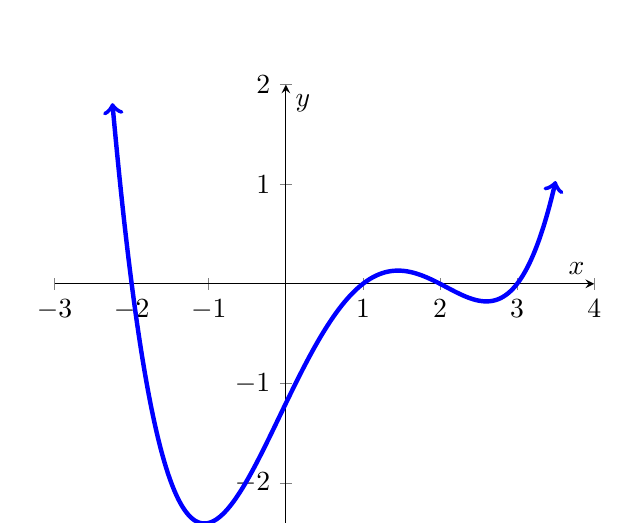
\begin{tikzpicture}
\begin{axis}[
    axis lines=middle,
    xmin=-3,xmax=4,
ymin=-2.5,ymax=2,
%   xtick={-6.28, -4.71,...,6.28},
%   ytick={-4, -3,...,4},
    xlabel={$x$},
    ylabel={$y$}
    ]
  \addplot[<->,domain=-2.25:3.5,blue, ultra thick, samples=500]  {0.1*(x+2)*(x-1)*(x-2)*(x-3)} ;
\end{axis}
\end{tikzpicture}
\end{center}

%absolute

\item For what value of $x$ does $s(x)$ have an absolute minimum on $[-2,3]$?

  \begin{enumerate}
  \item no absolute minimum
  \item $-2$
  \item $-1$ %correct
  \item $2.5$
  
  \end{enumerate}

%relative

\item For what value(s) of $x$ does $s(x)$ have a relative minimum on $[-2,3]$?

  \begin{enumerate}
  
  \item $-2.5, -0.25$ %gave y values instead
  \item $-1, 2.5$ %correct
  \item $1.5$ %rel max
  \item $2.5$ %did not include absolute too
  
  \end{enumerate}

%positive 

\item On what interval(s) is $s(x)$ positive? (Assume the function continues in the directions indicated.)
 
 
  \begin{enumerate}
  \item $(-\infty,-1) \cup (1.5,2.5)$ %decreasing
  \item $(-1,1.5) \cup (2.5,\infty)$ %increasing
  \item $(-\infty, -2) \cup (1,2) \cup (3,\infty)$ %correct, positive
  \item $(0,\infty)$ %positive x-values
  
    \end{enumerate}
    
%increasing

\item On what interval(s) is $s(x)$ increasing? (Assume the function continues in the directions indicated.)
 
 
  \begin{enumerate}
  %\item $(-\infty, -2) \cup (1,2) \cup (3,\infty)$ %positive
   \item $(-1, \infty)$
  \item $(-1,1.5) \cup (2.5,\infty)$ %correct, increasing
  \item $(-\infty,-1) \cup (1.5,2.5)$ %decreasing
  \item $(-\infty, -2) \cup (3,\infty)$ % just tails pointing up
   
    \end{enumerate}
 



\end{enumerate}


\end{document}


%old version below

% \documentclass{article}
% \usepackage[utf8]{inputenc}

% \usepackage[paperwidth=8.5in, paperheight=11in, top=1in, bottom=.5in, left=.5in, right=.5in]{geometry}
% \usepackage{fancyhdr, graphicx,tikz,amsmath,multicol,paracol}
% \usepackage[inline]{enumitem}
% \usepackage{tikz}
% \usepackage{pgfplots}
% \pgfplotsset{{compat=1.16},
% 	humanaxes/.style={axis lines=center, every axis plot/.append style={very thick, mark size=3}, x axis line style=-, y axis line style=-},
% 	humanaxeslabels/.style={every axis x label/.style={at={(current axis.right of origin)},anchor=west},every axis y label/.style={at={(current axis.above origin)},anchor=south}},
% 	human/.style={humanaxes, humanaxeslabels} }

% \pagestyle{fancy}
% \lhead{\large{\textbf{Module 3: Applications of Differentiation - Readiness Assurance Test}}}
% \chead{}
% \rhead{}
% \lfoot{}
% \cfoot{}

% %\rfoot{\thepage/\pageref{LastPage} }
% \setlength{\headheight}{14pt} %added in bc warning

% %%% The answers will be aligned to IF-AT Form B021, questions 31-40. 


% % 31 D
% % 32 C
% % 33 C
% % 34 A
% % 35 D
% % 36 D
% % 37 C
% % 38 A
% % 39 C
% % 40 D


% \begin{document}


% \begin{enumerate}


% % finding a derivative using the quotient rule

% \item Let $f(x)=\frac{x^2-2}{x+1}$. Find $f'(x)$.

%   \begin{enumerate}
  
  
%   \item $\frac{x^2+2x+2}{x+1}$ %no square in denominator
%   \item $\frac{3x^2+2x-2}{(x+1)^2}$ %forgot the minus in the quotient rule 
%   \item $\frac{-x^2-2x-2}{(x+1)^2}$ %wrong order in the quotient rule 
%   \item $\frac{x^2+2x+2}{(x+1)^2}$ %correct
%   \end{enumerate}

% % chain rule


% \item Let $g(x)=(x^2+x)^2$. Find $g'(x)$.

%   \begin{enumerate}
  
 
%   \item $2(x^2+x)^2(2x+1)$ %incorrect power rule
%   \item $2(x^2+x)$ %forgot chain rule 
%    \item $2(x^2+x)(2x+1)$ %correct
%   \item $(x^2+x)^2(2x+1)$ %no power rule 
%   \end{enumerate}

% % second derivative


% \item Let $t(x)=xe^x$. Find $t''(x)$.

%   \begin{enumerate}
  
 
%   \item $e^x (x+1) $ %first derivative
%   \item $xe^x $ %no derivative 
%    \item $e^x (x+2) $ %correct
%   \item $e^x$ %weird product rule 
%   \end{enumerate}



% % domain


% \item Let $h(x)=\frac{\sqrt{x+1}}{x^2-4}$. What is the domain of $g(x)$?

%   \begin{enumerate}
  
%   \item All real numbers $x \geq -1$ except $x=2$ %correct
%   \item All real numbers except $x=2$ %incorrect square, no square root
%   \item All real numbers except $x=\pm 2$ %no square root
%   \item All real numbers $x \geq -1$ %no denominator
%   \end{enumerate}

%  %zeros of polynomial
 
 
% \item Let $p(x)=(x-1)(x^2-5x+6)$. What are the zeros of $p(x)$?

%   \begin{enumerate}
  

%   \item $x= -1, -2, -3 $ %sign issue
%   \item $x= 1$ %no factoring
%   \item $x= 1, 5, 6$ %incorrect factoring 
%     \item $x= 1, 2, 3 $ %correct
%   \end{enumerate}
 

% % modelling with multiple variables


% \item A fashion designer has a budget of \$300 for fabric for a fabulous garment. The
% designer is going to use a combination of denim fabric which costs \$8 per yard and jersey fabric which costs \$12 per yard (partial yards are okay). Assume that the designer spends the entire budget of \$300 on these two fabrics. Let $J$ be the number of yards of jersey purchased and let $D$ be the number yards of denim purchased. Which of the following equations represents $J$ as a function of $D$?

%   \begin{enumerate}
  

%   \item $8J + 12D = 300$ %incorrect coefficients, no J in terms of D
%   \item $12J + 8D = 300$ %no J in terms of D
%   \item $J = \frac{300-12D}{8}$ %incorrect coeffiecients
%     \item $J = \frac{300-8D}{12}$ %correct
%   \end{enumerate}

% \pagebreak 

% %relative and absolute
 
% \item Let $s(x)$ be pictured below. When what are the relative and absolute minima of $s(x)$ on $[-2,3]$?

% \begin{center}
% \begin{tikzpicture}
% \begin{axis}[
%     axis lines=middle,
% %    xmin=-3,xmax=3,
% ymin=-2.5,ymax=2,
% %   xtick={-6.28, -4.71,...,6.28},
% %   ytick={-4, -3,...,4},
%     xlabel={$x$},
%     ylabel={$y$}
%     ]
%   \addplot[domain=-2.5:3,blue, ultra thick, samples=500]  {0.1*(x+2)*(x-1)*(x-2)*(x-3)} ;
% \end{axis}
% \end{tikzpicture}
% \end{center}

%   \begin{enumerate}

%   \item No absolute min, relative min at $x=-1, 2.5$ %incorrect absolute min
%    \item No absolute min, relative min at $x=-1, 1.5, 2.5$ %incorrect absolute min and max in there
%      \item Absolute min at $x=-1$, relative min at $x=-1, 2.5$ %correct
%   \item Absolute min at $x=-1$, relative min at $x=1.5, 2.5$ %max in there
%   \end{enumerate}

% %increasing vs positive 

% \item Consider the function $s(x)$ again (pictured above). On the interval $[-1,2]$, when is $s(x)$ positive and when is $s(x)$ increasing? 
 
 
%   \begin{enumerate}
%   \item Positive for $1<x<2$, increasing for $-1<x<1.5$ %correct
%   \item Positive for $x>0$, increasing for $-1<x<1.5$ %incorrect positive
%   \item Positive for  $1<x<2$, increasing for $-1<x<1$ %incorrect increasing
%   \item Positive for  $x>0$, increasing for $x>-1$ %incorrect both
 
%   \end{enumerate}
 



% \end{enumerate}


% \end{document}
